\documentclass{article}

\usepackage[a4paper, total={16cm, 28cm}]{geometry}
\usepackage{txfonts}
\usepackage{graphicx}
\usepackage{float}
\usepackage{hyperref}
\usepackage[figurename=Figura]{caption}

\author{Diego Antonio Román Cortés\\Profesor Guía: Rodrigo A. Vicencio}
\date{Departamento de Física, Facultad de Ciencias Físicas y Matemáticas, Universidad de Chile}
\title{Redes interorbitales basadas en moléculas fotónicas}

\begin{document} \maketitle
%Título del proyecto
%Nombre del candidato y del profesor guía o profesores guía

\section{Contexto del proyecto (introducción y descripción del estado del arte)}
	La técnica de escritura de guías de onda mediante el enfoque de láser de pulsos con duración temporal del orden de los femtosegundos dentro de vidrio borosilcato ha permitido la fabricación de redes fotónicas de variada índole \cite{bics, artificialFB}. Su importancia radica no sólo en emular situaciones propias de la física del sólido, sino que también en el estudio de fenómenos ópticos como la no-linearidad tipo Kerr.
	En particular, el acoplamiento interorbital SP \cite{interorbital} ha permitido el estudio de redes que presentan flujo magnético efectivo no trivial \cite{OAMcaging, ABCaging}. Recientemente se ha reportado la propagación de luz con momentum angular orbital (OAM) por medio de redes fotónicas que presevan simetría $C_3$ \cite{vortex}. El acoplamiento entre modos OAM permite la generación de flujos magnéticos complejos \cite{vortextrim}.
\section{Objetivos de la tesis}
\begin{enumerate}
	\item Utilizar moléculas fotónicas como base para fabricar y estudiar redes interorbitales.
	\item Entender el comportamiento de los modos guiados en moléculas fotónicas y su interacción en el régimen de acoplamiento débil.
\end{enumerate}
\section{Metodología}

Desde las ecuaciones de Maxwell en un medio dieléctrico no magnético sin cargas ni corrientes libres es posible escribir la siguiente ecuación asumiendo envolvente lenta $\textbf{E}(\textbf{r}) = \textbf{E}_1(\textbf{r}) e^{-i \textbf{k}_1 \cdot \textbf{r}}$.

\begin{equation}
	(\nabla-i\textbf{k}_1)\times(\nabla-i\textbf{k}_1)\times \textbf{E}_1 = k^2 \textbf{E}_1,
	 \label{eqn:maxwell}
\end{equation}
con $k \equiv k_0 n$.
La ecuación (\ref{eqn:maxwell}) es resuelta por el software comercial COMSOL y será una de las herramientas a usar en esta tesis. Por otro lado, utilizando la aproximación paraxial es posible simplificar la ecuación (\ref{eqn:maxwell}) y llegar a la implementación usual de los \textit{Beam Propagation Methods} usados ampliamente en el área \cite{bpm}.
\begin{equation}
	-i\lambdabar\frac{\partial}{\partial z}\psi(x,y,z) = \left(\frac{\lambdabar^2\nabla_\perp^2}{2n_0} + \Delta n(x,y)\right) \psi (x,y,z) \label{eqn:paraxial}
\end{equation}

Mientras que aplicando teoría acoplada de modos a la ecuación (\ref{eqn:paraxial}) para describir de forma discreta una red fotónica, es posible derivar las ecuaciones discretas tipo Schrödinger para la envolvente del campo eléctrico (\ref{eqn:CMT}):
\begin{equation}
	-i\frac{\partial u_{\vec{n}} }{\partial z} = \beta_{\vec{n}}u_{\vec{n}} + \sum_{\vec{m}\neq\vec{n}} C_{\vec{n},\vec{m}}u_{\vec{m}} \label{eqn:CMT}
\end{equation}

La excitación de redes fotónicas interorbitales hace necesario el uso de condiciones iniciales no triviales. Para ello se implementó una técnica de modulación espacial de luz que permite modular tanto la amplitud como la fase de el haz tipo gaussiano proveniente del láser \cite{slm}.

\begin{figure}[H]
	\centering
	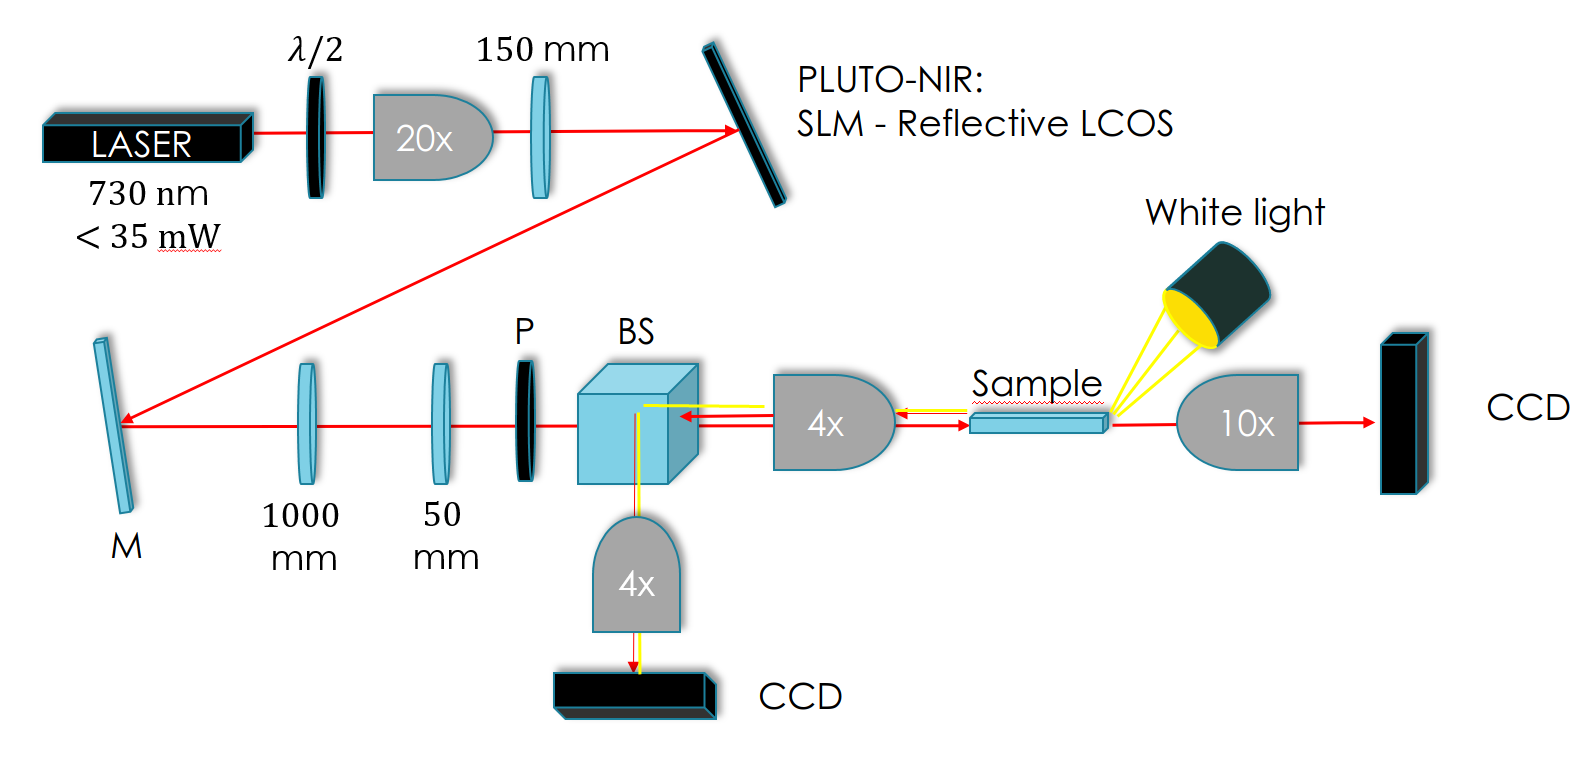
\includegraphics[width=0.9\linewidth]{./media/montaje.png}
	\caption{Montaje de excitación de guías de onda con condiciones iniciales moduladas en amplitud y fase.\label{fig:SLM}}
\end{figure}

\section{Trabajo adelantado (si lo hubiera)}

Durante el curso de Seminario de Investigación I (Primavera 2022) se hizo un barrido de parámetros de fabricación de guías de onda, en particular de potencia de escritura y separación entre guías, logrando la inversión de elipticidad el sintonizado de las constantes de propagación del modo fundamental $S$ de la molécula de excitación y el modo excitado $P_x$ de la molécula de acoplamiento.


\begin{figure}[H]
	\centering
	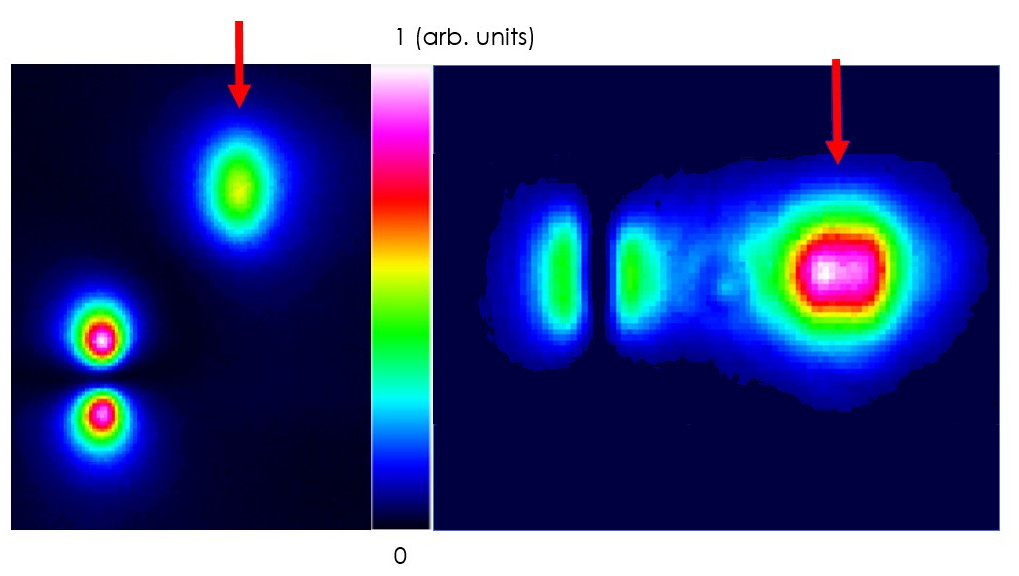
\includegraphics[width=0.5\linewidth]{./media/SPinteraction.jpg}
	\caption{Interacción interorbital en guías indivuduales y en moléculas fotónicas.}
\end{figure}

Durante el curso de Seminario de Investigación II (Otoño 2023) se implementó el montaje de modulación esquematizado en la Figura \ref{fig:SLM}. Con ello fue posible la excitación de un dipolo horizontal:

\begin{figure}[H]
	\centering
	\includegraphics[width=0.5\linewidth]{./media/dipole.png}
	\caption{Dímeros dipolares.}
\end{figure}

y de un OAM:

\begin{figure}[H]
	\centering
	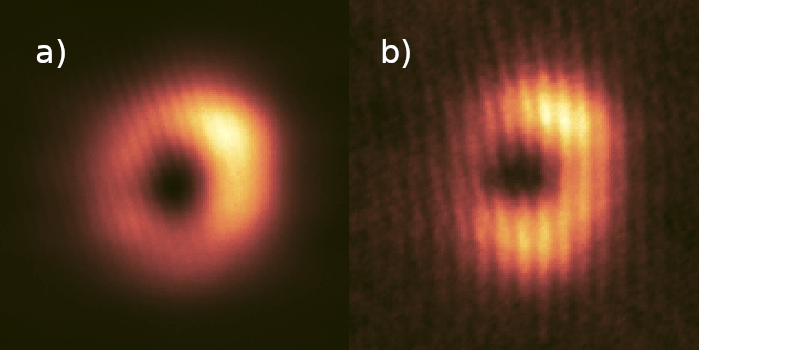
\includegraphics[width=0.5\linewidth]{./media/vortex.png}
	\caption{a) Intensidad de un OAM propagado en una molécula fotónica. b) Interferograma que captura el cambio de fase esperado.}
\end{figure}

\section{Plan de trabajo o carta Gantt}


% citations
\renewcommand\refname{Referencias}
\bibliographystyle{ieeetr}
\bibliography{citations}

\end{document}
